% Report source. Build from this folder: pdflatex report && bibtex report && pdflatex report && pdflatex report
\documentclass[12pt,a4paper]{article}
\usepackage[margin=1in]{geometry}
\usepackage[T1]{fontenc}
\usepackage{lmodern}
\usepackage{amsmath,amssymb}
\usepackage{graphicx}
\usepackage[font=footnotesize,labelfont=bf]{caption}
\setlength{\parindent}{0pt}
\setlength{\parskip}{0.4em plus 0.2em}
% let floats share pages with text instead of leaving half-empty pages
\renewcommand{\topfraction}{0.85}\renewcommand{\bottomfraction}{0.7}\renewcommand{\textfraction}{0.1}
\renewcommand{\floatpagefraction}{0.75}\setcounter{topnumber}{3}\setcounter{totalnumber}{4}
\setlength{\textfloatsep}{10pt plus 2pt minus 2pt}\setlength{\floatsep}{8pt plus 2pt minus 2pt}\setlength{\intextsep}{8pt plus 2pt minus 2pt}
\usepackage{url}
\usepackage[compact]{titlesec}
\usepackage[hidelinks]{hyperref}
\setcounter{secnumdepth}{0}
\let\oldthebibliography\thebibliography  % no extra space between references
\renewcommand{\thebibliography}[1]{\oldthebibliography{#1}\setlength{\itemsep}{0pt}}

\title{Which invariances survive implementation? \\ CMA-ES vs.\ Bayesian optimisation}
\author{Daniel Erbs Fodgaard, A0342235M \\ daniel\_fodgaard@u.nus.edu \\ \url{https://github.com/danielfodgaard/BOvsCMAES}}
\date{\vspace{-2.5em}}

\begin{document}
\maketitle

\section{Introduction}

Black-box optimisers such as Bayesian optimisation and CMA-ES never see the problem they are trying to optimise \cite{frazier2018, hansen2016}. The optimisers will only get back numbers from evaluations of the function they are trying to optimise. So even though a problem to be optimised might be described in different ways, e.g. in milliseconds or seconds, or on a rotated or logarithmic scale, this doesn't change the location of the optimum, and ideally it shouldn't change the behaviour of the solver either. I found it quite surprising that an optimiser's behaviour could change with how the problem is described, and even more surprising that solvers can be made invariant to these changes.

In Hansen's tutorial on CMA-ES he treats this as a design principle. He also lists the transformations CMA-ES is invariant to \cite{hansen2016}: strictly increasing transformations of \(f\), and linear transformations of the search space such as rescalings and rotations, provided the initial state is transformed accordingly. Bayesian optimisation, however, is built differently. It fits a Gaussian process to the values of \(f\), so how \(f\) is reported changes the model and potentially the search.

This raises a practical question: do these invariances actually hold in the implementations people use (pycma and BoTorch), and when they don't, what does it cost in terms of performance? In this report I test each invariance by running each method on a problem and on a transformed version of it with the same optimum, so any difference in performance is caused by the method.

\section{Background on the two methods}

CMA-ES samples \(\lambda\) points from \(N\left( m,\sigma^{2}C \right)\), ranks them by \(f\), and updates \(m\), \(\sigma\) and \(C\) from the ranked points only \cite{hansen2016}. So any strictly increasing \(g\) leaves the sequence of updates unchanged (but not necessarily what an implementation does with the values themselves, e.g. its termination criteria). Since the updates of \(m\) and \(C\) are equivariant under invertible linear maps of \(x\), a run on \(f(Ax)\) is the original run mapped by \(A^{- 1}\), provided the initial state (\(m_{0}\), \(\sigma_{0}\), \(C_{0}\)) is transformed with it. For a rotation the default \(C_{0} = I\) stays the same, so only \(m_{0}\) has to follow. For a rescaling \(\sigma_{0}\) has to be rescaled too.

Bayesian optimisation fits a Gaussian process (GP) \cite{frazier2018} to the observed values and chooses the next point by an acquisition function, here LogEI \cite{ament2023}, a numerically stable logarithm of expected improvement, which scores a point by how much the GP expects it to improve on the best value observed so far. The implementation I have chosen standardises the outputs, which makes it invariant to \(af + b\) with \(a > 0\), and uses an RBF kernel with one lengthscale per axis (ARD) whose prior assumes inputs in the unit cube. It also fits a noise variance even when \(f\) is noise-free, with a lower bound of \(10^{- 4}\) in standardised units. Nothing in it is invariant to a nonlinear \(g\) or to a rotation.

\section{Method setup}

\textbf{Paired design.} For every seed, method and setting I run the original and the transformed problem with the same random state and score both on the untransformed \(f\): \(f_{\text{best}}\) is the lowest untransformed \(f\) a run finds within its budget, and its level is \(\log_{10}f_{\text{best}}\).

\textbf{Problems.} Most experiments use the ellipsoid \(f(x) = \sum_{i}100^{(i - 1)/4}\left( x_{i} - x_{i}^{\ast} \right)^{2}\) in \(d = 5\) (condition number 100) on the box \(\lbrack - 5,5\rbrack^{5}\), with \(f^{\ast} = 0\) at an optimum \(x^{\ast}\) drawn uniformly in \(\lbrack - 2,2\rbrack^{5}\) (experiment 2 uses the sphere, and experiment 0's BO runs in \(d = 2\)). The seed fixes \(x^{\ast}\), the CMA-ES start point (uniform in the box unless stated) and BO's Sobol design, so they are shared by every transformation. Each experiment describes its own transformations, and the readme and script docstrings list every setting.

\textbf{Methods.} For CMA-ES I used pycma 4.5.0 with \(\sigma_{0} = 2.5\) (a quarter of the box width, as pycma's documentation recommends), population 8 (the default from \cite{hansen2016}), the box as bounds, and 2000 evaluations with all termination criteria off unless stated. For BO I used BoTorch 0.18.1 with \texttt{SingleTaskGP} defaults (ARD RBF, \texttt{Standardize}), inputs normalised to the box, LogEI \cite{ament2023}, and 10 Sobol points + 80 iterations unless stated. Budgets count objective evaluations, including the initial design, not model-fitting time.

\textbf{Why those implementations.} I chose BoTorch because it is a state-of-the-art BO library built on GPyTorch and PyTorch, both listed by Frazier \cite{frazier2018}, pycma because it is Hansen's own implementation, and Sobol points because Frazier recommends a space-filling initial design.

\textbf{Seeds and statistics.} Every result is the median over seeds (stated per experiment) of the best \(f\) after a fixed budget, or, where a lag matters, of the evaluations needed to reach a target (the measure COCO \cite{hansen2021coco} prefers), and the repository's \texttt{summary.csv} files add paired sign counts and Wilcoxon tests.

\textbf{Reproducibility.} Every experiment is one or two scripts in \texttt{code/} that write all CSVs and figures to \texttt{results/} (the readme maps experiments 0--5 to them, and the repository holds more results than fit here), and runs are deterministic given the seed, for BO bit for bit only on the same machine because some libraries use kernels specific to the CPU (MKL, OpenBLAS).

\section{Experiments and Results}

\subsection{\texorpdfstring{Experiment 0: Affine transforms \(af + b\) (control)}{Experiment 0: Affine transforms af + b (control)}}

First, I wanted to test the simplest invariance on Hansen's list, \(af + b\) with \(a > 0\), which both methods should have. CMA-ES has it because it only uses the ranking of the values and BO because \texttt{SingleTaskGP} standardises them. It also serves as a control for the experiments that follow: since \(af + b\) changes nothing that matters to either method, any difference between the runs can only come from floating-point rounding, which shows how much two runs of the same problem can differ by chance. Therefore I set it up such that both methods were run on the ellipsoid and on \(af + b\) for \(a \in \{ 10^{- 3},\allowbreak 1,\allowbreak 10^{3} \}\) and \(b \in \{ 0,\allowbreak 10^{3},\allowbreak 10^{8} \}\) with 5 seeds (CMA-ES in \(d = 5\) for 2000 evaluations, BO on the ellipsoid in \(d = 2\) with weights 1 and 100, for 40 evaluations, with EI and LogEI), and compared the internal state of every run with the run on \(f\) step by step.

\begin{figure}[htbp]
\centering
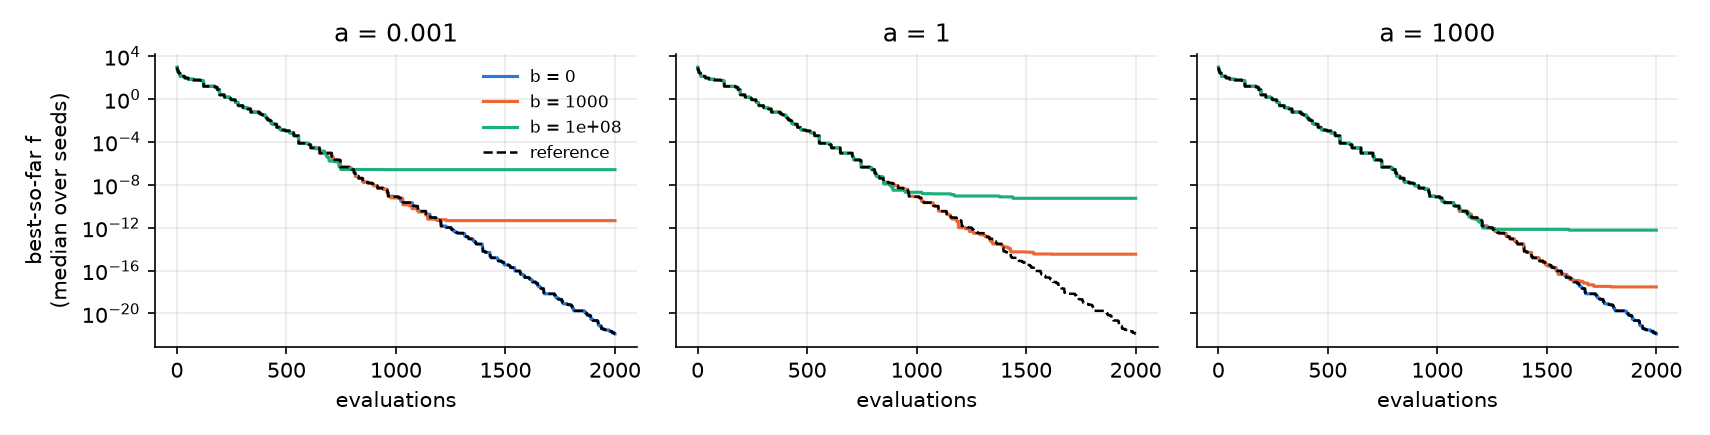
\includegraphics[width=0.7\textwidth]{figures/h1_cma.png}
\par\medskip
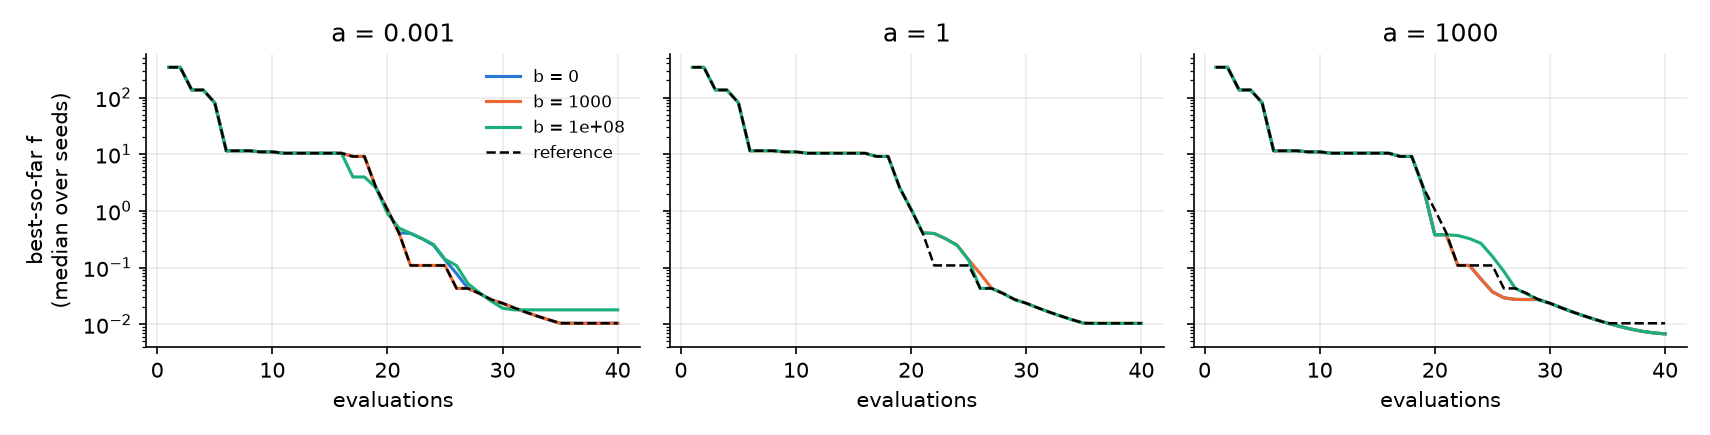
\includegraphics[width=0.7\textwidth]{figures/h1_bo.png}
\caption{E0. Median best-so-far \(f\) over 5 seeds on \(af + b\) (colours: \(b\)) against the run on \(f\) (dashed), for \(a = 10^{- 3},1,10^{3}\). Top: CMA-ES with a fixed budget. Bottom: BO with LogEI.}
\label{fig:e0}
\end{figure}

\textbf{Interpretation:}

For CMA-ES the run is identical to the run on \(f\) whenever \(b = 0\) (its curves lie exactly under the dashed reference in Figure~\ref{fig:e0}, top), and with \(b > 0\) it diverges. The reason is floating-point rounding: \(af + b\) only becomes a different problem once \(b\) is so large that the differences between values near the optimum fall below what \(af + b\) can resolve, and until then the ranking of the sampled points and therefore the run is the same.

For BO all curves stay close to the reference, whatever \(b\) is (Figure~\ref{fig:e0}, bottom), since within 40 evaluations BO only gets down to about \(f = 10^{- 2}\), far above the values where \(af + b\) starts to lose resolution. The runs still differ from the reference after a few iterations, because the GP fit and the acquisition optimiser amplify tiny rounding differences, so BO runs can only be compared as distributions of results, and as distributions they match.

Both results were expected, and the experiment served mostly as a sanity check. A natural next test was to go from affine to nonlinear monotone transforms \(g(f)\), to which CMA-ES should still be invariant and BO should not, which is experiment 1.

\subsection{\texorpdfstring{Experiment 1: Monotone transforms \(g(f)\)}{Experiment 1: Monotone transforms g(f)}}

For experiment 1 I wanted to test the invariance I was initially most surprised to read that CMA-ES had, but which makes a lot of sense once you know its internal workings: invariance to any strictly increasing \(g(f)\). CMA-ES should be exactly invariant to it because it uses ranks, while default BO, which models the values themselves, should not. However, instead of testing only default BO, I was inspired by Shirakawa \cite{shirakawa2016}, who made BO invariant to monotone \(g\) by fitting the GP to ranks. So I wanted to test how BO performs under rank transformations.

Therefore I set it up such that both methods were run on the ellipsoid under \(g \in \{ f^{1/4},\allowbreak f^{1/2},\allowbreak f^{2},\allowbreak f^{4},\allowbreak \log f,\allowbreak f/(f + 100),\allowbreak 1000f \}\), where \(1000f\) is an affine control, with 10 seeds. CMA-ES ran with a fixed budget of 2000 evaluations and with pycma's default stopping, and BO in three setups: default, the GP fitted to the ranks of \(g(f)\) \cite{shirakawa2016}, and the default with BoTorch's lower bound on the noise variance moved from \(10^{- 4}\) to \(10^{- 8}\). The low-noise setup came out of a first run, in which the fitted noise sat exactly at its lower bound, in units of \(f\) a noise of about 6, far larger than the best values BO finds, so the bound itself might keep BO from resolving the optimum.

\begin{figure}[htbp]
\centering
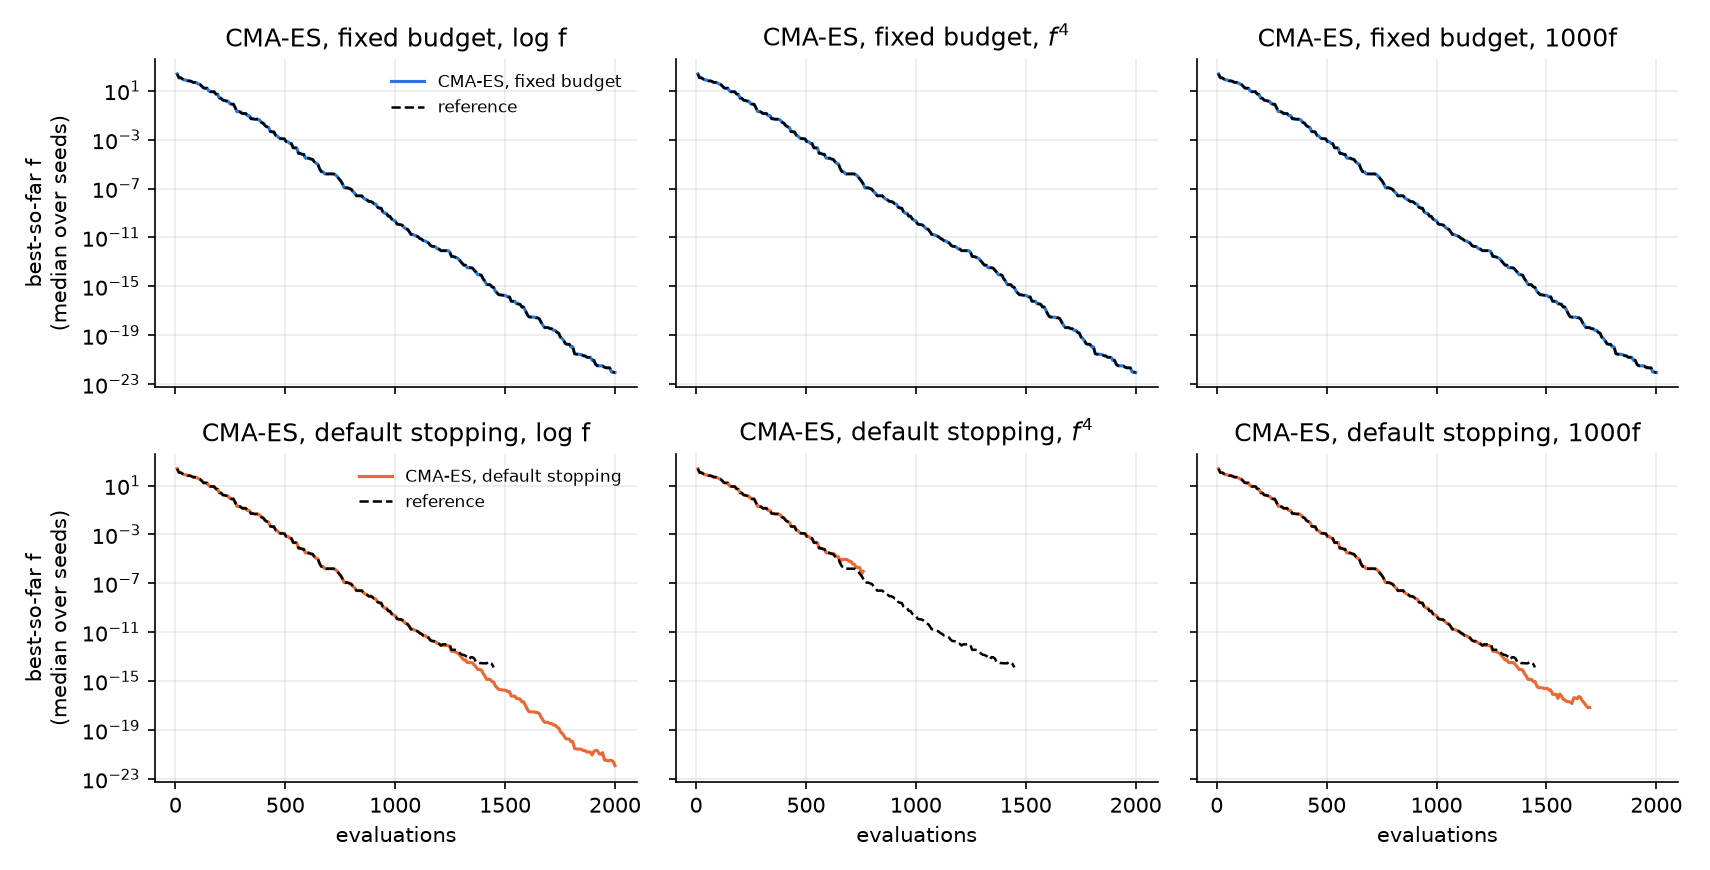
\includegraphics[width=0.6\textwidth]{figures/e1_cma.png}
\caption{E1, CMA-ES. Median best-so-far \(f\) over 10 seeds under three of the transforms against the run on \(f\) (dashed): one compressing (\(\log f\)), one expanding (\(f^{4}\)) and the affine control (\(1000f\)). Top: fixed budget. Bottom: pycma's default stopping.}
\label{fig:e1cma}
\end{figure}

\begin{figure}[htbp]
\centering
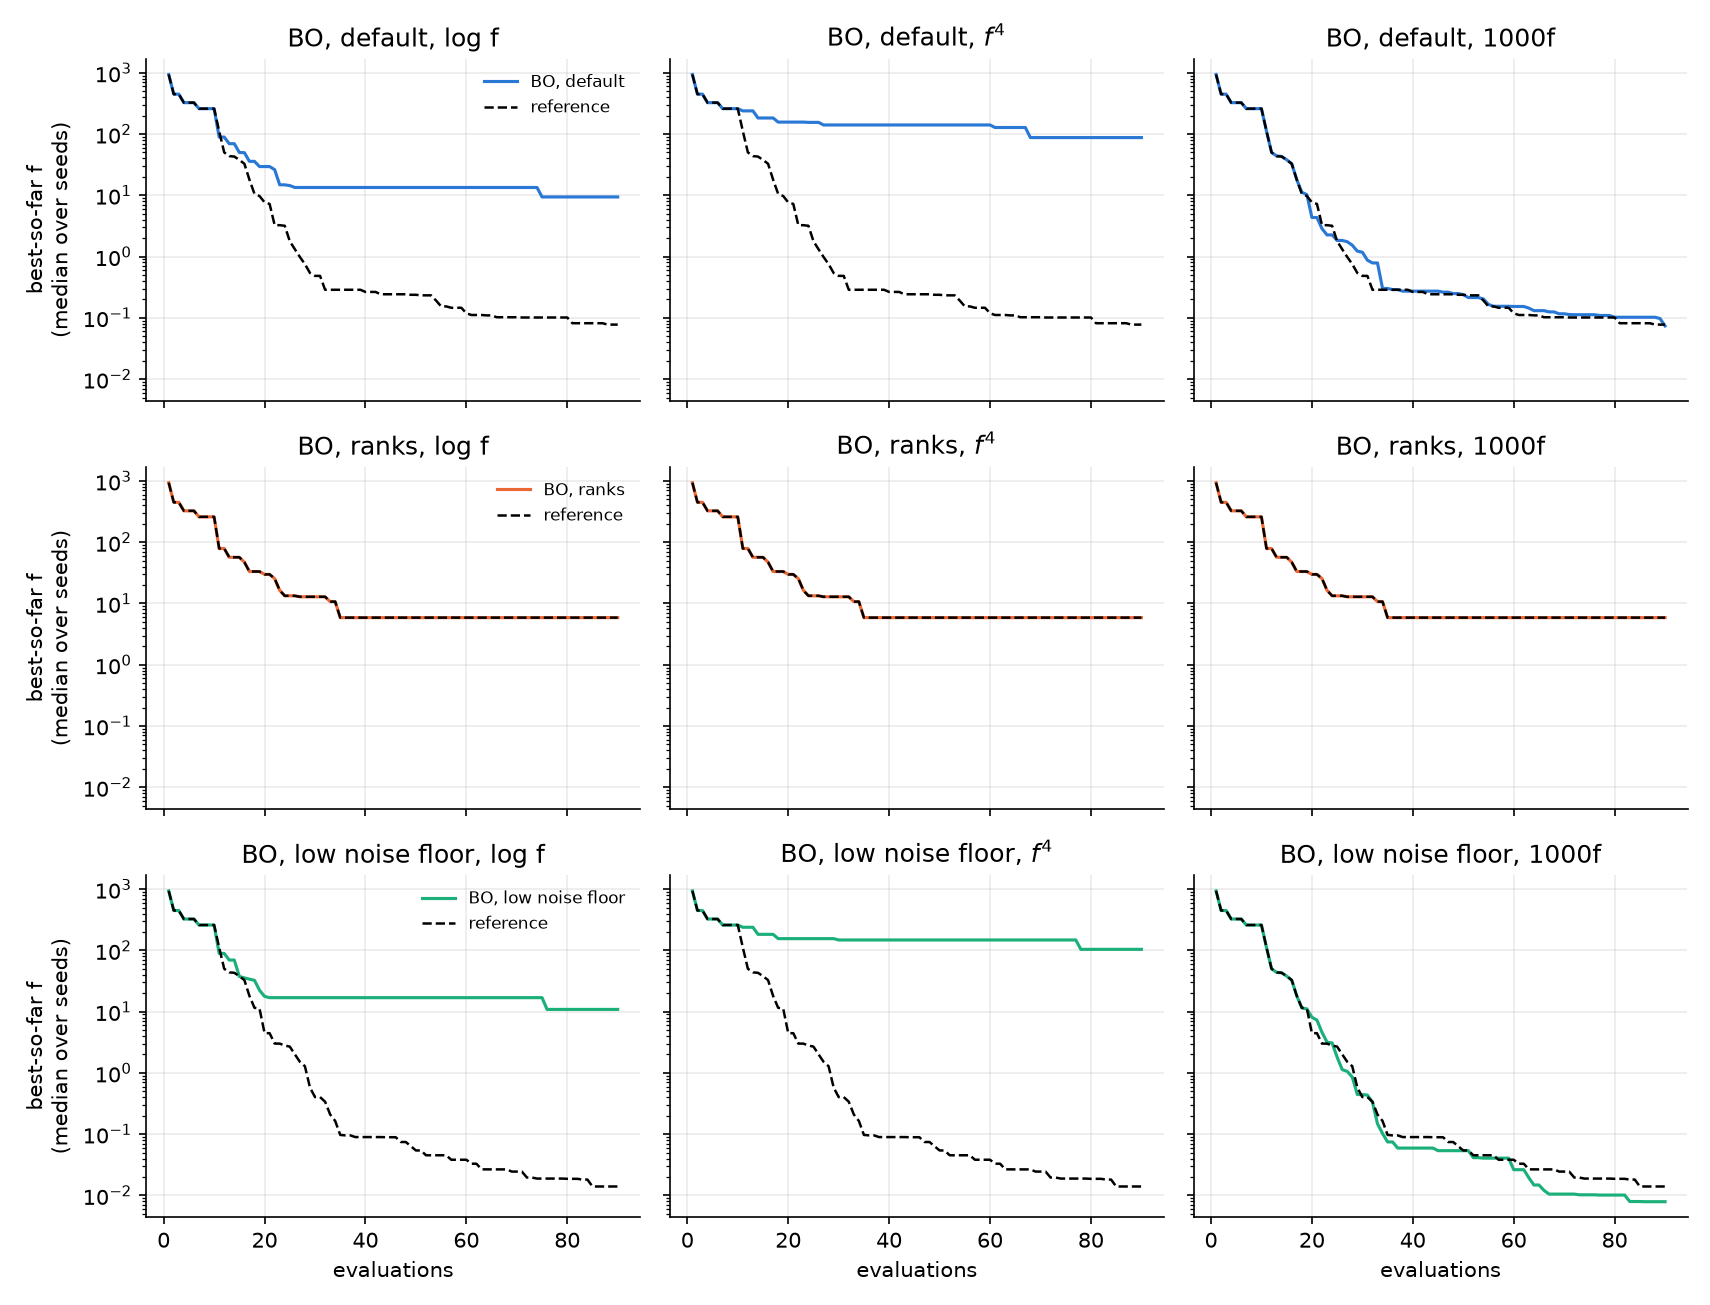
\includegraphics[width=0.55\textwidth]{figures/e1_bo.png}
\caption{E1, BO. Median best-so-far \(f\) over 10 seeds under the same three transforms, for default BO (top), BO on ranks (middle) and BO with a lower noise floor (bottom). The dashed reference in each row is that setup's own run on \(f\).}
\label{fig:e1bo}
\end{figure}

\textbf{Interpretation:}

After running the experiments I saw that the search of CMA-ES is invariant but its stopping rule is not (Figure~\ref{fig:e1cma}). With a fixed budget the curves for every \(g\) lie exactly on the reference (top row), but with default stopping the runs end at different points (bottom row): earlier on \(f^{4}\) and later on \(\log f\) and \(1000f\). The reason is that pycma's default stopping criterion \texttt{tolfun} compares absolute differences in \(g\), so it fires once the spread in \(f\) drops below about \(10^{- 11}/g\prime(f)\): early on \(f^{4}\), which is very flat near the optimum, later on \(1000f\), and never on \(\log f\), whose slope grows without bound near the optimum, so there the run continues until \texttt{tolx} or \texttt{tolxstagnation} fires or the 2000-evaluation cap is reached.

Default BO is not invariant (Figure~\ref{fig:e1bo}, top row): it follows the reference on \(1000f\), but on \(\log f\) and \(f^{4}\) its curves flatten after 20--30 evaluations and stay one to three orders of magnitude above the reference. Ranks (middle row) give exactly the same curve under every \(g\), so they do make BO invariant, but that curve flattens early too, about two orders of magnitude above default BO on \(f\). The low noise floor (bottom row) gets further on \(f\), but under \(\log f\) and \(f^{4}\) it stalls just like the default, so the noise floor is not what makes BO fail under a bad \(g\).

An explanation could be that the GP models the values it is given. A compressing \(g\) like \(\log f\) squeezes the deep, narrow minimum of the ellipsoid into a small change that the GP explains as noise, and an expanding \(g\) like \(f^{4}\) makes the function almost flat around the optimum and very steep far from it, so the GP ignores the flattest directions. In both cases the GP's picture of where the minimum lies is poor, the acquisition function stops finding improvements, and the curves flatten. Ranks remove the dependence on \(g\), but they also throw away how much better one point is than another, which is presumably the information default BO exploits on \(f\).

The invariance of the CMA-ES search was expected, but I was surprised that the invariance breaks in the stopping rule instead, by about 8 orders, and that for BO the invariant fix, ranks, costs about as much on \(f\) as a bad \(g\) costs default BO. A natural next test was the other family of invariances, transformations of \(x\), starting with a change of units, which is experiment 2.

\subsection{\texorpdfstring{Experiment 2: rescaling the axes of \(x\)}{Experiment 2: rescaling the axes of x}}

For the next experiment I wanted to test the invariance to a change of units. For CMA-ES it holds only if the initial state follows \cite{hansen2016}, i.e. if \(\sigma_{0}\) is scaled along, and BO should be unaffected as long as its inputs are normalised to the box. Therefore I set it up such that both methods were run on the sphere and on three copies of it in new units \(x = uz\) (per axis \(u_{i} = 10^{- (i - 1)/4}\), a factor 10 across the axes, and uniformly \(u = 0.01\) and \(u = 100\)), with the box, the optimum, the CMA-ES start and BO's Sobol design mapped along, so that each copy is the same problem. CMA-ES ran with its defaults (\(\sigma_{0} = 2.5\) in every unit) and with \(\sigma_{0}\) multiplied by \(u_{i}\) per axis (\texttt{CMA\_stds}, on the ellipsoid with the per-axis copy's factors), the same without bounds, and with pycma's per-coordinate step-size cap switched off. BO ran with \texttt{Normalize} and on raw inputs. CMA-ES used 50 seeds, BO used 10. As a side case I also kept the box and stretched only \(f\), which gives the ellipsoid: a harder problem (condition number 100), not a relabelling.

\begin{figure}[htbp]
\centering
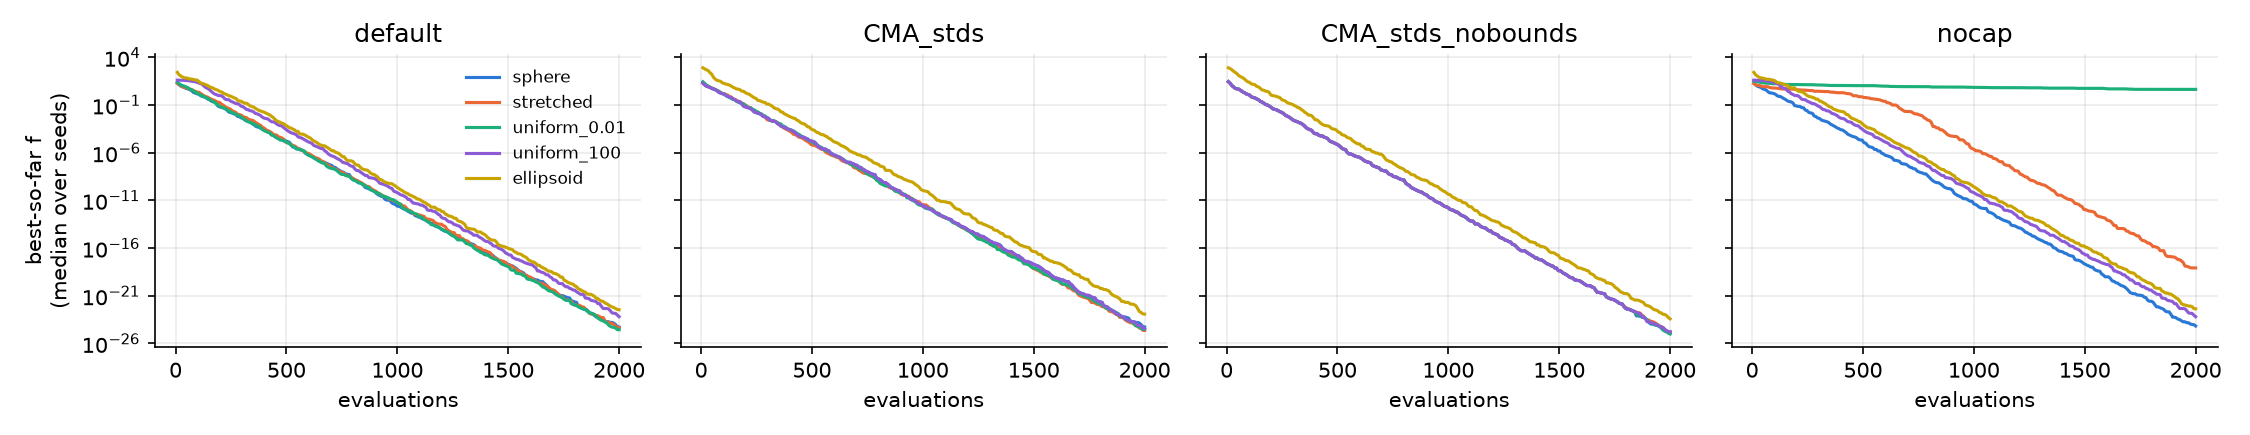
\includegraphics[width=0.82\textwidth]{figures/e2_cma.png}
\par\medskip
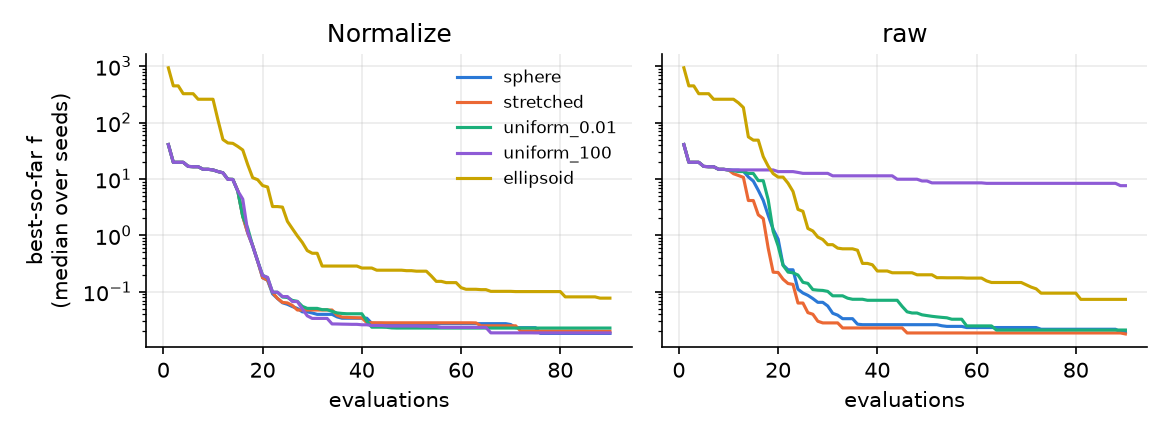
\includegraphics[width=0.45\textwidth]{figures/e2_bo.png}
\caption{E2. Median best-so-far \(f\) on the sphere, its three rescaled copies and the ellipsoid (same box, condition number 100). Top: CMA-ES per setup, 50 seeds. Bottom: BO with inputs normalised to the box (\texttt{Normalize}) and on raw inputs, 10 seeds.}
\label{fig:e2}
\end{figure}

\textbf{Interpretation:}

After running the experiments I saw that both methods are invariant to a change of units as long as they are given the new scale: CMA-ES through \(\sigma_{0}\) scaled along with the units (\texttt{CMA\_stds}), and BO through inputs normalised to the box (\texttt{Normalize}) (Figure~\ref{fig:e2}). With \texttt{CMA\_stds}, with and without bounds, the curves for all four versions of the sphere lie on top of each other. With the defaults the copy in units 100 times larger lags behind, the copy in units 0.01 does not, and the per-axis copy lags only two to three generations (about 20 evaluations). With the cap switched off the copy in units 0.01 never gets going and the per-axis copy is much slower than the sphere. BO with \texttt{Normalize} gives the same curve on all copies of the sphere, and on raw inputs only the copy in units 100 times larger stalls. The ellipsoid, which keeps the box and only stretches \(f\), is a genuinely harder problem for both methods.

The reason for the default CMA-ES result is pycma's step-size cap (\texttt{maxstd\_boundrange}): it caps each coordinate's standard deviation at a third of that coordinate's box width, so the box itself tells pycma the scale. The cap can shrink a too-large \(\sigma_{0}\) but not grow a too-small one, and at \(u = 100\), \(\sigma_{0} = 2.5\) is 100 times too small. With the cap off nothing corrects \(\sigma_{0}\), which at \(u = 0.01\) is 100 times too large and per axis 10 times too large on the stiffest axis. For raw-input BO at \(u = 100\) the box is 1000 wide while the GP's lengthscale starts at 0.458, its prior's mode, so the GP sees no correlation between any two points and never learns anything about the function.

The invariance with \texttt{CMA\_stds} was expected from Hansen's argument, but I was surprised that the default run is almost unaffected when the units shrink: the box does the experimenter's job of setting the scale, but only in one direction. A natural next test from Hansen's list was rotation, which is experiment 3.

\subsection{\texorpdfstring{Experiment 3: rotating \(x\)}{Experiment 3: rotating x}}

I wanted to test the rotation invariance in my next experiment, which CMA-ES should have (only its start has to be rotated along) and BO's ARD kernel, with one lengthscale per axis, should not. Therefore I set it up such that both methods were run on the ellipsoid and on the same function in rotated coordinates, \(f\left( R^{T}y \right)\) with a random rotation \(R\) per seed, keeping the box at \(\lbrack - 5,5\rbrack^{5}\) and rotating the CMA-ES start along (drawn from the ball of radius 5, so that it stays in the box). CMA-ES ran with the default box handling, with the per-coordinate cap off, and with no bounds (50 seeds). BO with the default ARD kernel and with an isotropic RBF kernel (one lengthscale) as the control, for 150 evaluations (10 seeds).

\begin{figure}[htbp]
\centering
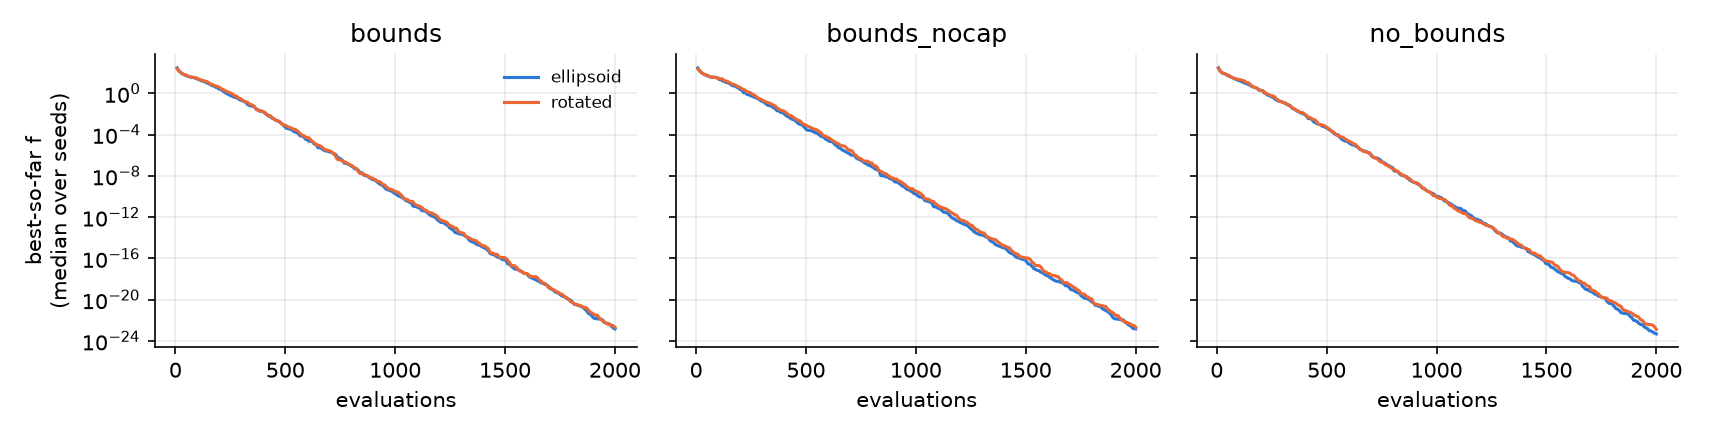
\includegraphics[width=0.82\textwidth]{figures/e3_cma.png}
\par\medskip
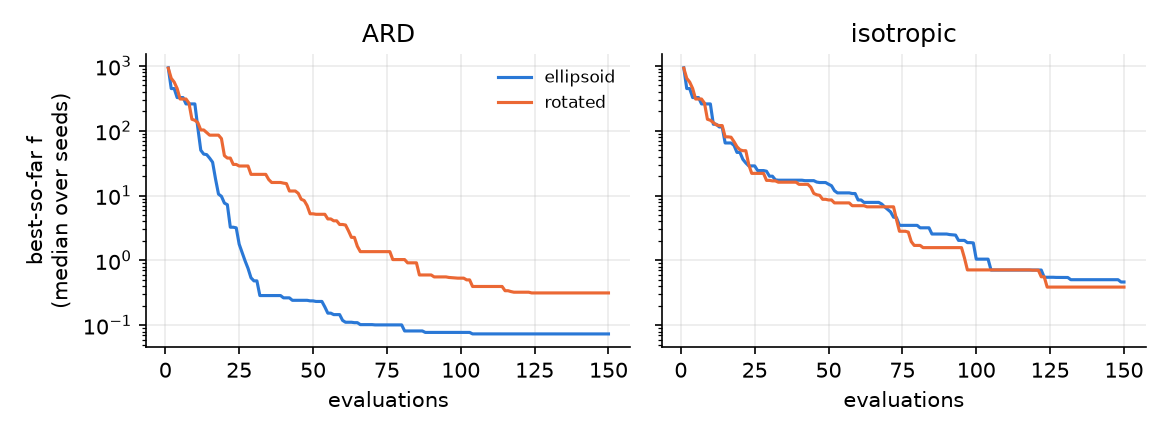
\includegraphics[width=0.5\textwidth]{figures/e3_bo.png}
\caption{E3. Median best-so-far \(f\) on the ellipsoid and its rotated version. Top: CMA-ES with the default box handling, with the per-coordinate cap off, and without bounds, 50 seeds. Bottom: BO with the default ARD kernel (left) and an isotropic RBF kernel (right), 10 seeds.}
\label{fig:e3}
\end{figure}

\textbf{Interpretation:}

After running the experiments I saw that CMA-ES is rotation-invariant, with or without bounds: in every setup the curves for the ellipsoid and its rotated version lie on top of each other (Figure~\ref{fig:e3}, top). The rotated runs only lag a little behind, by up to three generations (up to 22 evaluations) with bounds and at most about one generation without. Default BO, on the other hand, notices the rotation (Figure~\ref{fig:e3}, bottom left): the rotated problem is clearly worse after 90 evaluations, and by 150 it has only partly caught up. An explanation could be the ARD kernel. On the ellipsoid the fitted lengthscales follow the axis weights, but after rotation no axis is special and they collapse to similar values.

The BO result was expected, but I was surprised by the price of the fix: the isotropic kernel (bottom right) treats both problems alike, but it is much worse than ARD on the ellipsoid and no better than ARD even on the rotated problem. For CMA-ES I had expected the coordinate-wise box handling to cost something measurable under rotation, and it costs only this small lag. This confirms Hansen's claim from his list of invariances, up to a small boundary effect.

\subsection{Following up}

Of the transformations in experiments 0--3, the monotone transformations of experiment 1 were by far the most costly for BO, and unlike a change of units, which normalising the inputs removes, they have no fix that comes for free, since ranks cost about two orders of magnitude on \(f\) itself. That made them the most natural direction to follow up, and raises the opposite question: instead of making BO blind to the representation, can BO find a good representation of \(f\) by itself? In a black-box setting the values we get back might well be a transformed version of a function that a GP models much better, and since evaluations, not GP fits, are the expensive part, BO can afford to try out transformations of the values it has already seen without spending a single extra evaluation.

Any such output transformation needs two things: a family of transformations to choose from, and a criterion for choosing among them. I tested the two ends of that trade-off. Experiment 4 uses an advanced family with a simple criterion: the learned output transformation of HEBO \cite{hebo2022}, a state-of-the-art BO method (in the literature also called output warping \cite{snelson2004}), which can use any power of the values and picks the one that makes the values look normally distributed. Experiment 5 uses a simple family with an advanced criterion: a handful of fixed transformations, judged by how well the GP itself can predict the data after each of them. If only one of them gets back to the level of default BO on \(f\), it tells us whether the family or the criterion is what counts.

\subsection{Experiments 4 and 5: learning or choosing the output transformation}

Both experiments run BO on the problems from experiment 1 (experiment 5 on five of them), with the same seeds and initial designs (10 seeds, and 30 on \(f + 1000\) and \(f - 10\), run by the follow-up script \texttt{followup.py}), and change only what the GP is fitted to. In experiment 4 the GP is fitted to a Box-Cox power transformation of the observed values (Yeo-Johnson when a value is not positive, as in HEBO), whose power is refitted every iteration so that the transformed values look as normally distributed as possible. Box-Cox needs positive values and is singular at zero, so its result depends on where the zero of \(f\) is, and I also ran it on the shifted problems \(f + 10\), \(f + 1000\) and \(f - 10\). In experiment 5 one GP is fitted for each candidate transformation (a few powers, \(\log\) and \(\exp\)), and the one whose GP best predicts each observed value from the others (leave-one-out cross-validation \cite{rasmussen2006}, an idea going back to Jones et al. \cite{jones1998}) proposes the next point. It either chooses again every iteration or chooses once, after the initial design. Its candidates can undo \(f^{4}\) and \(\log f\), but not \(f/(f + 100)\).

\begin{figure}[htbp]
\centering
\begin{minipage}[t]{0.45\textwidth}\centering
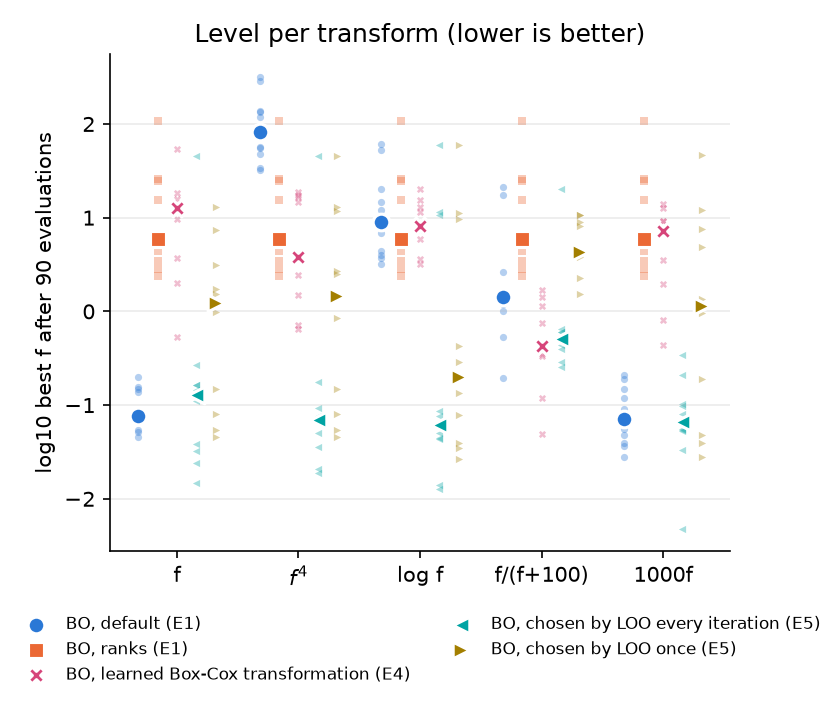
\includegraphics[width=1.00\linewidth]{figures/d_level.png}
\end{minipage}\hfill
\begin{minipage}[t]{0.45\textwidth}\centering
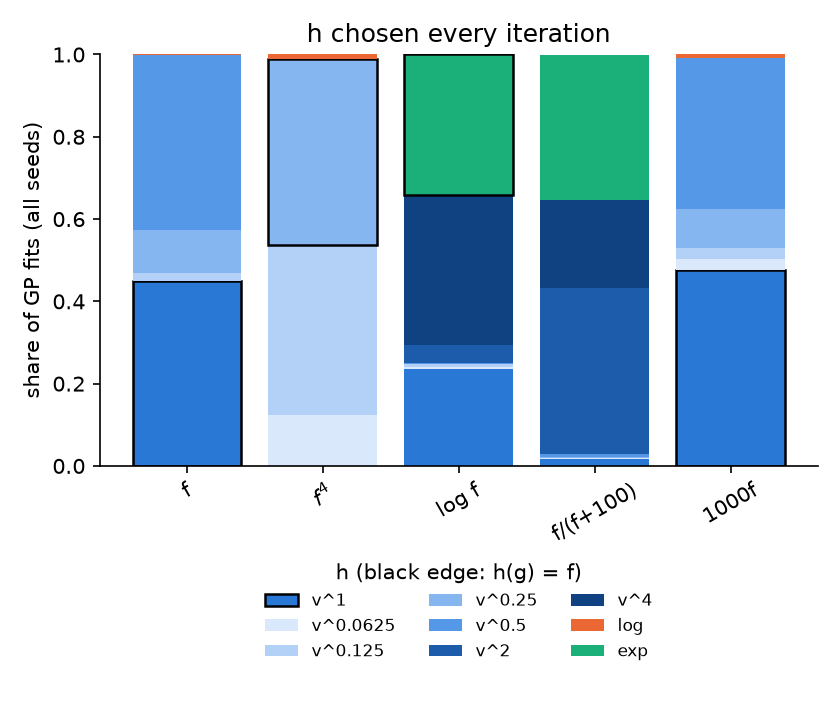
\includegraphics[width=1.00\linewidth]{figures/d_choices.png}
\end{minipage}
\caption{E4 and E5. Left: \(\log_{10}\) best untransformed \(f\) after 90 evaluations per \(g\) and setup: default BO and ranks (E1), the learned Box-Cox transformation (E4), and the transformation chosen by leave-one-out every iteration or once (E5). Small markers are seeds, large markers medians. Right: which transformation \(h\) of the observed values \(v = g(f)\) E5 chose when choosing every iteration. Each bar is one \(g\), and the colours show how often each \(h\) was chosen, as a share of all GP fits over all seeds. A black edge marks the \(h\) that turns \(g\) back into \(f\). For example, on \(f^{4}\), \(h = v^{0.25}\) gives back \(f\) and \(v^{0.125}\) gives \(\sqrt{f}\).}
\label{fig:e45}
\end{figure}

\textbf{Interpretation:}

After running the experiments I saw two very different outcomes (Figure~\ref{fig:e45}, left). The learned transformation of experiment 4 lands close to the ranks under almost every \(g\): it is roughly invariant to \(\log f\) and the powers of \(f\), but about two orders worse than default BO on \(f\) itself. Experiment 5, choosing every iteration, lands where default BO does on \(f\) under every \(g\) it can undo, including \(f^{4}\) and \(\log f\), where default BO itself fails badly. A few seeds end much worse, so this holds for the typical run rather than for every run. Where no candidate undoes \(g\) (\(f/(f + 100)\)), experiment 5 does not get back to the level of \(f\), and choosing only once after the initial design is worse than choosing every iteration on most \(g\).

An explanation for the difference could be how each experiment judges a transformation. Experiment 4 picks the transformation that makes the values look normally distributed, which on these problems is close to a logarithm: the same kind of compressed representation that made default BO fail in experiment 1. Experiment 5 instead asks which transformation lets the GP predict the data best. On \(f^{4}\) both families contain the exact inverse, so there the criterion alone makes the difference, and the GP's own criterion wins. Interestingly, experiment 5 picks the transformation that turns \(g\) back into exactly \(f\) in less than half of its fits (Figure~\ref{fig:e45}, right)! On most \(g\) it switches between \(f\) and its square root, and that is enough. The shifted problems show a weakness of experiment 4 on top of that: because Box-Cox is singular at zero, \(f + 1000\) and \(f - 10\) give quite different results, which default BO would not.

I expected experiment 4, with the more advanced family, to get back to the level of default BO on \(f\), since it can represent the inverse of every power of \(f\). So I was surprised that it ended up as costly as ranks, and that experiment 5 works without finding \(f\). The answer to the question from the previous section is therefore that the criterion might count more than the family, at least when it is applied every iteration: chosen only once, the GP's own criterion is not clearly better than experiment 4 on \(f^{4}\). That leaves the question of how these costs compare with simply using CMA-ES at the same budget, which is taken up in the discussion section.

\section{Conclusion}

\textbf{CMA-ES invariances:} For CMA-ES, the invariances hold where Hansen's argument applies, the update equations, and leak only where it does not: through floating-point resolution under a large shift, through the stopping rule under a monotone \(g\), and through the box handling under a change of units. The box cuts both ways: pycma's per-coordinate step-size cap supplies the scale when the user's \(\sigma_{0}\) is too large but not when it is too small (experiment 2), while under rotation the bounded runs lag only slightly more than the unbounded ones (experiment 3).

\textbf{BO invariances:} For BO, the invariances it has come from preprocessing (\texttt{Standardize}, \texttt{Normalize}). The invariances it lacks can be bought, but ranks and the learned transformation of experiment 4 both cost about two orders of magnitude on \(f\), most likely because each settles on one representation that is worse than \(f\) on this problem. The default presumably wins on \(f\) because it exploits the structure it is given, such as the axis-aligned scales that experiment 3's rotation removes, while CMA-ES gets its invariances free because it never used that information. Experiment 5 points to a third option: re-selecting the representation every iteration by the GP's own predictive fit kept the typical level of default BO wherever the inverse was among the candidates, while selecting once did not. That is robustness, not invariance, and only as good as the candidate set.

\section{Discussion}

\textbf{BO against CMA-ES at the same budget:}

A direct comparison of the two methods does not make much sense. They are built for very different regimes: BO spends a lot of computation on each evaluation and is meant for budgets of tens to hundreds of evaluations, while CMA-ES needs little computation per evaluation but thousands of evaluations, and the two start from different information (10 space-filling Sobol points against one start point and \(\sigma_{0}\)). So the comparison below is not a 1-to-1 ranking of the methods. I use CMA-ES as a yardstick for invariance: its result does not depend on \(g\) at all, so comparing with it at BO's own budget shows how much of BO's advantage survives when the representation changes.

At 88 evaluations of experiment 1, CMA-ES is at a median \(f\) of about 50, the same under every \(g\), while default BO after 90 evaluations is between two and a half and three orders of magnitude better on \(f\). A bad representation eats that lead: under \(f^{4}\) default BO ends behind CMA-ES. Ranks and the transformations of experiments 4 and 5 all stay ahead of CMA-ES under every \(g\), experiment 5 by about the full lead where it can undo \(g\). In other words, BO's advantage at a small budget comes from exploiting the representation it is given, and the same dependence is what makes it fragile: when the representation is bad, a method that ignores it entirely can do better. The invariant and adaptive variants give up part of BO's best case in exchange for not losing everything in the worst case.

\textbf{Limitations:} All experiments use smooth, noise-free quadratics, mostly in five dimensions, with default settings, so the size of BO's costs may well differ on other problems, while the leaks of CMA-ES (a stopping rule that compares absolute differences and a box handling that acts per coordinate) should carry over. With only 10 BO seeds the medians are themselves uncertain (single seeds often spread over an order of magnitude, Figure~\ref{fig:e45}), the candidate set of experiment 5 was chosen knowing which \(g\) it would be tested on, and a trust-region BO such as TuRBO \cite{eriksson2019} was not tested.

\textbf{On the use of AI:}

Throughout this project AI (Claude from Anthropic) has been used for idea generation, coding, debugging, active learning and writing. I have mostly used it to help with the implementation of experiments I have set up. This has helped me run more tests and better experiments because setting up an experiment and iterating on it is faster. I am responsible for the content and quality of the submitted work.

\nocite{frazier2018,hansen2016,eriksson2019,hansen2021coco}
{\footnotesize
\bibliographystyle{ieeetr}
\bibliography{refs}
}
\end{document}
